\documentclass[12pt]{article}
\usepackage{xr}
\externaldocument{"../Book_II/chapter_6"}
\externaldocument{"../Book_II/chapter_8"}

\usepackage[a4paper, margin=1in]{geometry}
\usepackage{tikz}
\usetikzlibrary{positioning, arrows.meta, decorations.pathreplacing, calc, backgrounds}
\usepackage{amsmath,amssymb}
\usepackage{hyperref}
\usepackage{amsthm}
\usepackage{pdflscape} % For the landscape environment

\usepackage[margin=1in]{geometry}
\usepackage{amsmath,amssymb,amsthm,amsfonts}
\usepackage{graphicx}
\usepackage{hyperref}
\usepackage{enumitem}
\setlist[enumerate]{align=left,labelindent=0pt}
\hypersetup{colorlinks=true, linkcolor=blue, urlcolor=blue, citecolor=blue}

% Chapter-specific theorem environments
\theoremstyle{definition}
\newtheorem{definition}{Definition}[section]
\newtheorem{remark}{Remark}[section]
\theoremstyle{plain}
\newtheorem{theorem}{Theorem}[section]
\newtheorem{axiom}{Axiom}[section]
\newtheorem{lemma}{Lemma}[section]
\newtheorem{proposition}{Proposition}[section]
\newtheorem{corollary}{Corollary}[section]

\title{\textbf{Chapter 1: Fundamental Decomposition of Simple Test}}
\author{Dmytro Surdu}
\begin{document}
\maketitle

\section{Test Primitives}
\label{sec:test-primitives}

Throughout this chapter a \emph{test} is a sextuple
\[
  \mathfrak T = \bigl(\mathcal M,\;\mathcal Z^{\rm in},\;\mathcal Z^{\rm out},\;U,\;E,\;\mathcal S\bigr),
\]
where $\mathcal M,\mathcal Z^{\rm in},\mathcal Z^{\rm out}$ are compact metric spaces, $U:\mathcal M\times\mathcal Z^{\rm in}\to\mathcal M$ and $E:\mathcal M\to\mathcal Z^{\rm out}$ are continuous, and $\mathcal S=\{\varepsilon_n\}_{n\ge1}$ is a (minimal) Certification Standard (Book II, Chapter 8, Def.~\ref{def:minimal-standard}).  We now fix \emph{three} primitive constructions over the input time-domain \(\mathfrak{D}_{IN}\) that will be used to build all composite tests in this book.  All the definitions below are stated directly in terms of maps and guard‑bands.

Our three primitives are selected to build a Turing Machine. The Turing machine is selected because of its generality; indeed, no counterexample for the Church-Turing thesis based on a non-exotic (i.e., based on arguably complete theories - no quantum gravity and black hole paradoxes) physical process that doesn't require a physically infinite precision and/or physically infinite computing power is known. 

The implications of the current work are interesting for further exploration of the Church-Turing thesis violations, and we will discuss them later.

\section{Preliminaries: What Counts as a Valid Test?}
\label{sec:valid-test}

\begin{definition}[Valid Test]
\label{def:valid-test}
A \emph{test} is a sextuple
\[
  \mathfrak T = \bigl(\mathcal M,\;\mathcal Z^{\rm in},\;\mathcal Z^{\rm out},\;U,\;E,\;\mathcal S\bigr)
\]
satisfying the following axioms:

\begin{enumerate}[label=(VT\arabic*)]
  \item \textbf{Compact continuity.} 
        $\mathcal M,\mathcal Z^{\rm in},\mathcal Z^{\rm out}$ are compact metric spaces and 
        $U:\mathcal M\times\mathcal Z^{\rm in}\to\mathcal M$, 
        $E:\mathcal M\to\mathcal Z^{\rm out}$ are continuous.

  \item \textbf{Reachable invariant basin.}
        There exists a nonempty compact set $\mathcal B\subseteq\mathcal M$ such that
        (i) every trajectory enters $\mathcal B$ in finite time, and
        (ii) $\Theta\in\mathcal B \Rightarrow U(\Theta,z)\in\mathcal B$ for all admissible $z$ (invariance).

  \item \textbf{Minimal certification standard.}
        $\mathcal S=\{\varepsilon_n\}_{n\ge1}$ is a nonincreasing sequence $\varepsilon_n\downarrow0$ such that each
        $\varepsilon_n$ is the infimum radius simultaneously ensuring (a) forward robustness and (b) completeness of the index‑$n$ certification procedure.

  \item \textbf{Shell forward‑closure.}
        Writing $\mathcal B_n=\{\Theta:\operatorname{dist}(\Theta,\mathcal B)\le\varepsilon_n\}$,
        we have for all $n$:
        \[
          \Theta\in\mathcal B_n,\ z^{\rm in}\in U(\Theta,\cdot)^{-1}(\mathcal B_n)
          \ \Longrightarrow\ 
          U(\Theta,z^{\rm in})\in\mathcal B_n.
        \]

  \item \textbf{Polynomial reachability (for NP–certifiability).}
        There exists a polynomial $p$ such that every trajectory enters $\mathcal B$ by time
        $T_{\max}\le p(\lvert\text{input}\rvert)$.  (This axiom can be omitted if one studies certifiability independently of complexity class.)
\end{enumerate}
\end{definition}

\begin{remark}
Conditions (VT1)–(VT4) encapsulate the physical/epistemic regularity needed to talk about guard‑bands and robustness. (VT5) is only required when we later connect certifiability to NP; the structural results (finite guarded decomposition, aspect uniqueness) use only (VT1)–(VT4).
\end{remark}

\subsection{The Primitive–Global Standard Equivalence}
\label{subsec:primitive-global-equivalence}
The very first question in building any decomposition is to find a way to distribute the Certification Standard. We can show that the \emph{minimality} of the Certification Standard $\mathcal{S}$ is enough to allow an equivalent distribution.

\begin{theorem}[Primitive–Global Certification Standard Equivalence]
\label{thm:primitive-global-equivalence}
Let 
\[
  \mathfrak T=(\mathcal M,\mathcal Z^{\rm in},\mathcal Z^{\rm out},U,E,\mathcal S)
\]
be a valid test (Def.~\ref{def:valid-test}) with invariant, reachable basin \(\mathcal B\) and minimal global Certification Standard  (Def.~\ref{def:minimal-standard}, Book II, Chapter 8)
\(\mathcal S=\{\varepsilon_m\}_{m\ge1}\), giving shells \(\mathcal B_m=\{\Theta:\operatorname{dist}(\Theta,\mathcal B)\le\varepsilon_m\}\).
Assume $U$ admits, at level $m$, a **finite open partition** 
\[
\mathcal Z^{\rm in}=\bigsqcup_i N_i
\] 
and define the restricted maps 
\[
U_i:=U\!\mid_{\mathcal M\times N_i}
\].

Then the following are equivalent:

\begin{enumerate}[label=\textup{(\alph*)}, leftmargin=2em]
  \item \textbf{Global minimal forward‑closure:}  
  \(\varepsilon_m\) is the minimal radius such that for every \(\Theta\in\mathcal B_m\) and every \(z\in\mathcal Z^{\rm in}\) satisfying
  \(d\bigl(z,\partial N_{i(z)}\bigr)\ge\varepsilon_m\) we have \(U(\Theta,z)\in\mathcal B_m\).
  
  \item \textbf{Existence of minimal local radii:}  
  There exist branchwise (minimal) radii \(\{\varepsilon_{m,i}\}_{i=1}^k\) with
  \[
    \forall\,\Theta\in\mathcal B_m,\ \forall\,z\in N_i:\ 
       d\bigl(z,\partial N_i\bigr)\ge\varepsilon_{m,i}\ \Longrightarrow\ 
       U_i(\Theta,z)\in\mathcal B_m,
  \]
  such that 
  \[
    \varepsilon_m=\min_{1\le i\le k}\varepsilon_{m,i},
  \]
  and no strictly smaller family \(\{\varepsilon'_{m,i}<\varepsilon_{m,i}\}\) preserves the above property for branch \(i\).
\end{enumerate}
\end{theorem}

\begin{proof}
We prove \((a)\Rightarrow(b)\) and \((b)\Rightarrow(a)\).

\medskip
\noindent\(\boxed{(b)\Rightarrow(a)}\)  
Given the local radii, set \(\varepsilon_m=\min_i\varepsilon_{m,i}\).  
For any \(\Theta\in\mathcal B_m\) and \(z\in\mathcal Z^{\rm in}\) with branch \(i(z)\) and 
\(d(z,\partial N_{i(z)})\ge\varepsilon_m\), we also have \(d(z,\partial N_{i(z)})\ge\varepsilon_{m,i(z)}\), so
\[
  U(\Theta,z)=U_{i(z)}(\Theta,z)\in\mathcal B_m.
\]
Thus \(\varepsilon_m\) enforces global forward‑closure.  
Minimality carries over: if a smaller \(\widehat\varepsilon_m<\varepsilon_m\) sufficed globally, it would undercut at least one branch’s minimal \(\varepsilon_{m,j}\), contradicting its minimality.

\medskip
\noindent\(\boxed{(a)\Rightarrow(b)}\)  
This is the “necessity” (upward) direction.

\smallskip
\emph{Step 1: Define local candidates.}  
Fix \(m\) and branch \(i\).  
For each \(\Theta\in\mathcal B_m\), consider the set
\[
  R_{m,i}(\Theta)
  := \bigl\{\,r>0 : \forall\,z\in N_i,\ d(z,\partial N_i)\ge r \Rightarrow 
      U_i(\Theta,z)\in\mathcal B_m \bigr\}.
\]
By assumption (a) at the global level, \(\varepsilon_m\) enforces forward‑closure; in particular, for every \(\Theta\in\mathcal B_m\) and every \(z\in N_i\) with \(d(z,\partial N_i)\ge\varepsilon_m\), we have \(U_i(\Theta,z)=U(\Theta,z)\in\mathcal B_m\).  
Hence \(\varepsilon_m\in R_{m,i}(\Theta)\), so \(R_{m,i}(\Theta)\neq\varnothing\).

Define the \emph{pointwise minimal} radius
\[
  \varepsilon_{m,i}^\Theta := \inf R_{m,i}(\Theta),
\]
and then take
\[
  \varepsilon_{m,i} := \sup_{\Theta\in\mathcal B_m}\varepsilon_{m,i}^\Theta.
\]
Because \(\mathcal B_m\) is compact and \(U_i\) is continuous, a standard compactness argument (finite subcover over \(\mathcal B_m\)) shows that \(\varepsilon_{m,i}<\infty\) and the supremum is attained (or can be approximated arbitrarily closely).  Thus \(\varepsilon_{m,i}\) is well-defined and finite.

\smallskip
\emph{Step 2: Local forward‑closure.}  
Let \(\Theta\in\mathcal B_m\), \(z\in N_i\), and assume \(d(z,\partial N_i)\ge\varepsilon_{m,i}\).  
By definition of \(\varepsilon_{m,i}\), for every \(\delta>0\) there exists \(\Theta'\in\mathcal B_m\) with \(\varepsilon_{m,i}^{\Theta'}>\varepsilon_{m,i}-\delta\), so for any \(r<\varepsilon_{m,i}\) and any such \(\Theta'\),
\[
  d(z,\partial N_i)\ge r \ \Longrightarrow\ U_i(\Theta',z)\in\mathcal B_m.
\]
Continuity of \(U_i\) in \(\Theta\) (and closedness of \(\mathcal B_m\)) allows us to pass to the limit \(\Theta'\to\Theta\), ensuring
\(U_i(\Theta,z)\in\mathcal B_m\).  
Hence each \(\varepsilon_{m,i}\) enforces (\(\star\)).

\smallskip
\emph{Step 3: Equality of minima.}  
Since \(\varepsilon_m\) guarantees global closure, any \(z\) with
\(d(z,\partial N_{i(z)})\ge\varepsilon_m\) is admissible at its branch.
Therefore, for each \(i\),
\[
  \varepsilon_{m,i}\;\le\;\varepsilon_m.
\]
Consequently,
\[
  \min_i\varepsilon_{m,i}\;\le\;\varepsilon_m.
\]
On the other hand, if 
\(\min_i\varepsilon_{m,i}<\varepsilon_m\),
then \(\varepsilon_m\) would not be minimal globally: we could choose
\(\widehat\varepsilon_m:=\min_i\varepsilon_{m,i}\)
and still have forward‑closure everywhere, contradicting (a).  
Thus \(\varepsilon_m=\min_i\varepsilon_{m,i}\).

\smallskip
\emph{Step 4: Local minimality.}  
If some branch radius could be lowered strictly, say \(\varepsilon'_{m,j}<\varepsilon_{m,j}\) still satisfying (\(\star\)), then the new global minimum 
\(\min(\varepsilon'_{m,j},\min_{i\neq j}\varepsilon_{m,i})\) would be \(<\varepsilon_m\), violating global minimality in (a).  
Hence each \(\varepsilon_{m,i}\) is minimal.

\smallskip
We have constructed minimal local radii whose minimum equals \(\varepsilon_m\).  
This completes \((a)\Rightarrow(b)\).

\medskip
\noindent\textbf{Conclusion.}  
Both directions hold, yielding the stated equivalence.
\end{proof}

\begin{remark}[Reading the Equivalence]
The theorem formalizes a “meet–distribute” duality:
\begin{itemize}
  \item Starting from branchwise tolerances (local standards), you \emph{meet} them to get the global minimal standard.
  \item Starting from a global minimal standard, you \emph{distribute} it down to each branch, obtaining minimal local standards whose meet is the original one.
\end{itemize}
Thus the Certification Standard is neither purely global nor purely local—it is the fixed point of this meet–distribute process.
\end{remark}

\begin{lemma}[Minimal Standard $\Rightarrow$ Boundary Margin]
\label{lem:no-crossing-from-minimal}
Assume Theorem~\ref{thm:primitive-global-equivalence} and let the finite tick-$m$ partition be $\mathcal Z^{\rm in}=\bigsqcup_{i=1}^k N_i$ with branchwise minimal radii $\{\varepsilon_{m,i}\}$ and global minimal $\varepsilon_m=\min_i\varepsilon_{m,i}$. Define the \emph{certified input core} of branch $i$ by
\[
  C_{m,i}\ :=\ \{\, z\in N_i : d(z,\partial N_i)\ge \varepsilon_{m,i}\,\}.
\]
Then for every $\Theta\in\mathcal B_m$ and $z\in C_{m,i}$ we have
\[
  U_i(\Theta,z)\in\mathcal B_m,
\]
and, in particular, any certified trajectory that stays in $C_{m,i}$ cannot cross $\partial N_i$ in one step. Moreover, the global certified core $C_m:=\bigsqcup_i C_{m,i}$ is open and nonempty in each branch.
\end{lemma}

\begin{proof}
By Theorem~\ref{thm:primitive-global-equivalence}(b), $d(z,\partial N_i)\ge \varepsilon_{m,i}$ implies $U_i(\Theta,z)\in\mathcal B_m$ for all $\Theta\in\mathcal B_m$. The definition of $C_{m,i}$ gives the claimed inclusion. Openness/nonemptiness follow because each $N_i$ is open and $\varepsilon_{m,i}>0$ is minimal; trimming by a positive margin leaves a nonempty open subset.
\end{proof}

\subsection{Sequential Test}
\label{subsec:sequential}

\begin{definition}[Sequential Composition]
Let
\[
  \mathfrak T'=(\mathcal M,\mathcal Z^{\rm in},\mathcal Z^{\rm mid},U',E',\mathcal S')\quad\text{and}\quad
  \mathfrak T''=(\mathcal M,\mathcal Z^{\rm in},\mathcal Z^{\rm out},U'',E'',\mathcal S'')
\]
share the same state space $\mathcal M$ and input space $\mathcal Z^{\rm in}$.  
Their \emph{Sequential Test} is
\[
  \mathfrak T_{\rm seq}
  =(\mathcal M,\mathcal Z^{\rm in},\mathcal Z^{\rm out},U_{\rm seq},E_{\rm seq},\mathcal S_{\rm seq}),
\]
where
\[
  U_{\rm seq}(\Theta,z)=U''\bigl(U'(\Theta,z),z\bigr),
  \qquad
  E_{\rm seq}(\Theta)=E''(\Theta),
\]
and the standard can be taken as
\[
  \varepsilon_n^{\rm seq}=\min(\varepsilon'_n,\varepsilon''_n).
\]
\end{definition}

\begin{lemma}[Metric Compatibility for Sequential Composition]
\label{lem:seq-metric-compat}
Let $(\mathcal{Z}^{\mathrm{out}},d_{\mathrm{out}})$ be the output space of the first primitive and $(\mathcal{Z}^{\mathrm{in}},d_{\mathrm{in}})$ the input space of the second, and let $T:\mathcal{Z}^{\mathrm{out}}\to\mathcal{Z}^{\mathrm{in}}$ be the connecting map. If $T$ is Lipschitz with constant $L_T<\infty$, then any tolerance $\varepsilon$ in $(\mathcal{Z}^{\mathrm{in}},d_{\mathrm{in}})$ corresponds to tolerance $L_T^{-1}\varepsilon$ in $(\mathcal{Z}^{\mathrm{out}},d_{\mathrm{out}})$. In particular, on compact metric spaces, $L_T$ is finite, so branchwise minimal tolerances can be transported uniformly between primitives.
\end{lemma}

\begin{proposition}
If $\mathfrak T'$ and $\mathfrak T''$ are valid tests, then $\mathfrak T_{\rm seq}$ is a valid test.  Continuity and forward‑closure are preserved under the chosen $\mathcal S_{\rm seq}$.
\end{proposition}

\begin{proof}
Composition of continuous maps is continuous.  Guard‑band radii shrink to the minimum to guarantee both stages remain inside their respective shells; thus forward‑closure holds.  Minimality of $\mathcal S_{\rm seq}$ follows by the same argument (cannot enlarge either constituent without breaking soundness).
\end{proof}

\subsection{Conditional Test}
\label{subsec:conditional}

\begin{definition}[Conditional Test]
Let $\{N_i\}_{i=1}^k$ be a finite open partition of $\mathcal Z^{\rm in}$ and suppose we have $k$ update maps
\[
  U_i:\mathcal M\times N_i\to\mathcal M
  \qquad\text{and a common emission}\quad E:\mathcal M\to\mathcal Z^{\rm out}.
\]
Define
\[
  U_{\rm cond}(\Theta,z)=U_i(\Theta,z)\quad\text{if }z\in N_i,
\]
and set $\mathfrak T_{\rm cond}=(\mathcal M,\mathcal Z^{\rm in},\mathcal Z^{\rm out},U_{\rm cond},E,\mathcal S_{\rm cond})$ with
\[
  \varepsilon_n^{\rm cond} := \min_{1\le i\le k}\varepsilon_{n,i},
\]
where $\varepsilon_{n,i}$ guarantees forward‑closure for branch $i$.
\end{definition}

\begin{proposition}
If each branch $(\mathcal M,N_i,\mathcal Z^{\rm out},U_i,E,\mathcal S_i)$ is a valid test on its domain $N_i$, and trajectories never cross the boundaries $\partial N_i$ once certified (guard‑bands leave margins), then $\mathfrak T_{\rm cond}$ is a valid test.
\end{proposition}

\begin{proof}
$U_{\rm cond}$ equals $U_i$ on $N_i$, preserving continuity there.  Guard‑band margins ensure no reachable trajectory hits $\partial N_i$.  Taking the minimum radius preserves forward‑closure on all branches simultaneously, and minimality is inherited (any larger radius would violate some branch).
\end{proof}

%================== Loop‑Until Test (Revised & Expanded) ==================
\subsection{Loop‑Until Test}
\label{subsec:loop}

We now give a precise definition of the \emph{Loop‑Until} test, making explicit its dependence on the primitives (\textsc{Conditional}, \textsc{Sequential}) and on the inductive guarded decomposition (Theorem~\ref{thm:inductive-decomposition}).

\begin{definition}[Loop‑Until Test]
\label{def:loop-until}
Let
\[
  \mathcal S=\{\varepsilon_n\}_{n\ge1}, 
  \qquad
  \mathcal B_n=\bigl\{\Theta:\mathrm{dist}(\Theta,\mathcal B)\le\varepsilon_n\bigr\},
\]
and let for each $n$ the depth‑$n$ {\upshape Conditional} map
\[
  U^{(n)}:\mathcal M\times\mathcal Z^{\rm in}\longrightarrow \mathcal M
  \quad\text{(Theorem~\ref{thm:inductive-decomposition})},
\]
which itself is built by nesting \textsc{Sequential} and \textsc{Conditional} primitives on the cells $N^{(n)}_{\mathbf i}$.  Define the \emph{Loop‑Until} state‑update
\[
  \widetilde U\;:\;(\mathcal M\times\mathbb N)\times\mathcal Z^{\rm in}
  \;\longrightarrow\;\mathcal M\times\mathbb N
\]
by
\[
  \widetilde U\bigl((\Theta,n),\,z\bigr)
  =
  \begin{cases}
    \bigl(U^{(n)}(\Theta,z),\,n\bigr), 
    & \Theta\notin\mathcal B_n, \\[6pt]
    \bigl(\Theta,\,n+1\bigr), 
    & \Theta\in\mathcal B_n\ \text{(advance level or halt if $n$ final)}.
  \end{cases}
\]
\noindent

That is, the update first applies $U^{(n)}$ at the current depth $n$ and checks membership in $\mathcal{B}_n$; only upon success is $n$ incremented (or the test halted if the target basin $\mathcal{B}$ has been reached).

More formally, the \emph{Loop-Until Test} operates as follows:
\begin{itemize}
  \item It reads an \emph{input stream} $\{z_0,z_1,\dots\}$ in discrete ticks $t=0,1,2,\dots$.
  \item It maintains an internal pair $(\Theta_t,n_t)$, where $\Theta_t\in\mathcal M$ is the current belief-state and $n_t\in\mathbb N$ is the current shell index, initialized to $(\Theta_0,1)$.
  \item At each tick $t$:
    \begin{enumerate}
      \item Apply the depth-$n_t$ update map to obtain
      \[
         \Theta_{t+1} \;=\; U^{(n_t)}(\Theta_t,\,z_t).
      \]
      \item \textbf{Check for level completion:} If $\Theta_{t+1}\in\mathcal B_{n_t}$, then
        \begin{enumerate}
          \item If $\mathcal B_{n_t}$ is the final target basin $\mathcal B$, emit $E(\Theta_{t+1})$ and halt.
          \item Otherwise, advance the shell index by setting $n_{t+1} := n_t+1$.
        \end{enumerate}
      \item If $\Theta_{t+1}\notin\mathcal B_{n_t}$, keep the same shell index by setting $n_{t+1} := n_t$.
    \end{enumerate}
\end{itemize}
In this form, the membership test is always performed against the same shell $\mathcal B_{n_t}$ that the depth-$n_t$ map is guaranteed (by the inductive decomposition) to reach in a single tick, preserving the one-tick-per-level progress property.

Its \emph{input time‑domain} is the full measurement stream \(\{z_t\}\); its \emph{output time‑domain} is exactly the single tick at which it halts.
\end{definition}


\subsection{Closure Under Composition}

\begin{proposition}[Primitive Closure]
\label{prop:primitive-closure}
The class of valid tests is closed under any finite nesting and composition of the two primitives: Sequential and Conditional.
\end{proposition}

\begin{proof}
Induct on the composition tree.  Each primitive preserves continuity, compactness, forward‑closure of shells (with appropriately chosen $\varepsilon_n$), and minimality (by taking minima where necessary).  Therefore any finite composite is a valid test.
\end{proof}

\subsection{How to prove Loop-Until Test Validity?}
Loop-Until Test we defined above iterates over the Sequential and Conditional Tests. There are no worries about the former; however, recall the validity proposition of the latter:
\begin{quote}
    If each branch $(\mathcal M,N_i,\mathcal Z^{\rm out},U_i,E,\mathcal S_i)$ is a valid test on its domain $N_i$, 
\end{quote}
\begin{quote}
\underline{and trajectories never cross the boundaries $\partial N_i$ once certified (guard‑bands leave margins),}
\end{quote}
\begin{quote}
then $\mathfrak T_{\rm cond}$ is a valid test.
\end{quote}
Therefore, in order to construct a valid Loop-Until Test, we \emph{must} ensure the underlined condition is satisfied.

The weakest necessary axiom is this direct underlined statement itself, formulated in a set-theoretic form below.


\subsection{Axiom: Input‑Traceability / Open‑Preimage}
\label{subsec:axiom-input-traceability}

\begin{axiom}[Input‑Traceability / Open‑Preimage]
\label{ax:open-preimage}
Let $\mathfrak T=(\mathcal M,\mathcal Z^{\rm in},\mathcal Z^{\rm out},U,E,\mathcal S)$ be a valid test (Def.~\ref{def:valid-test}), and let $\mathcal B_n=\{\Theta:\operatorname{dist}(\Theta,\mathcal B)\le\varepsilon_n\}$ be the $n$‑th shell induced by the (minimal) Certification Standard $\mathcal S$.  We postulate:
\[
  \forall\,n\ge1,\ \forall\,\Theta\in\mathcal M:\quad
  U(\Theta,\cdot)^{-1}(\mathcal B_n)
  \ \text{is open and nonempty in }\mathcal Z^{\rm in}.
\]
\end{axiom}

\paragraph{Interpretation.} 
This axiom ensures that for every certification shell and every state:
(i) there \emph{exists} at least one admissible input that drives the next state into the shell (nonemptiness = existential controllability), and 
(ii) admissibility is robust to small perturbations of that input (openness = guard‑band margin in input space).  
It is precisely what allows us to \emph{trace back} the certification constraint on state space to concrete, well‑behaved input conditions—hence the name “Input‑Traceability.”

\subsubsection*{Two Variants of Traceability Assumptions}

We now distinguish two variants explicitly:

\begin{definition}[PL-Traceability / Path-Local Input-Traceability]
\label{pl-traceability}
For each fixed \(\Theta\in\mathcal M\) and shell index \(n\), the preimage \(U(\Theta,\cdot)^{-1}(\mathcal B_n)\) is nonempty and open. This is the minimal input-traceability assumption used to certify \emph{realized} execution paths locally.
\end{definition}

\begin{definition}[UI-Traceability / Universal Input-Traceability]
\label{def:ui-traceability}
PL-Traceability holds, and additionally
\[
\bigcup_{\Theta\in\mathcal M} U(\Theta,\cdot)^{-1}(\mathcal B_n)=\mathcal Z^{\mathrm{in}},
\]
i.e., every input lies in some open preimage of the basin. Under this stronger assumption one can extract a global finite guarded partition of \(\mathcal Z^{\mathrm{in}}\) at tick 0.
\end{definition}
\begin{remark}[Scope of Traceability Assumptions]
In Chapters~1--2 we work under \emph{UI-Traceability} (Def.~\ref{def:ui-traceability}) to obtain \emph{global} finite guarded decompositions with short proofs. In Chapter~3 we weaken this to \emph{PL-Traceability} (Def.~\ref{pl-traceability}) and recover the Fundamental Test Equivalence via the ATRT Theorem, showing that UI is not essential, reflecting the metrological practice. We call this out here so every global decomposition result in this chapter can assume UI-Traceability \emph{explicitly}.
\end{remark}



\subsection{Corollary: Analogy to Classical Traceability}
\label{subsec:traceability-analogy}

\begin{corollary}[Structural Traceability Chain]
\label{cor:traceability-analogy}
Under the hypotheses of Theorem~\ref{thm:primitive-global-equivalence}, the family of local standards $\{\mathcal S^{(i)}\}_i$ forms a finite “traceability chain” for $\mathcal S$: every certified result can be referenced—via the finite decomposition tree—to a sequence of local tolerances whose meet equals the global tolerance. 

This mirrors (but is not identical to) classical metrological traceability:
\begin{enumerate}
  \item \textbf{Hierarchy of tolerances.} Local $\varepsilon_{n,i}$’s play the role of uncertainty allocations at each comparison step.
  \item \textbf{Finite chain.} Compactness + open‑preimage ensure finitely many branches (no infinite regress).
  \item \textbf{Unbroken linkage.} Guard‑band forward‑closure guarantees no gap in the logical chain from input admissibility to final certified state.
\end{enumerate}
\end{corollary}

\begin{proof}
Each certified emission is produced at a leaf or node of the finite decomposition tree.  Tracing upward, its admissibility rests on local radii at each branch it traversed. Taking the minimum across siblings preserves global robustness. Thus the certified output is “covered” by a finite set of local tolerances whose conjunction equals the global one—exactly the notion of a structural traceability linkage. 
\end{proof}

\begin{remark}[Difference from Institutional Traceability]
Classical traceability involves referencing measurements to national/international standards through documented calibrations over time. Our “traceability” is structural and topological: it references the \emph{Certification Standard} down to input conditions through the update map. The analogy is conceptual (hierarchical propagation of uncertainty/tolerance), not institutional.
\end{remark}



%================== Loop‑Until Test Validity (Revised Proof) ==================
\subsection{Loop‑Until Test Validity}
\label{subsec:loop-until-validity}

\begin{proposition}[Validity of the Loop-Until Test]
\label{prop:loop-until-valid-test}
Under VT1–VT4 of Definition~\ref{def:valid-test}, \textbf{VT2 (Reachable invariant basin)}, and the Input-Traceability / Open-Preimage Axiom~\ref{ax:open-preimage}, the Loop-Until Test (Definition~\ref{def:loop-until}) is itself a valid test and halts in finite time.
\end{proposition}

\begin{proof}
We prove validity by reducing \emph{Loop‑Until} to a finite sequential composition of one‑tick tests, each of which is valid by the primitives.

\smallskip\noindent\textbf{Step 1: One‑Tick Test Validity.}  
Fix any shell index $n\ge1$.  By Axiom~\ref{ax:open-preimage} and compactness of $\mathcal Z^{\rm in}$, Theorem~\ref{thm:inductive-decomposition} produces a finite guarded decomposition
\[
  \mathcal Z^{\rm in}
  \;=\;\bigsqcup_{\mathbf i\in I_n}N^{(n)}_{\mathbf i},
  \quad
  U^{(n)}\bigl|_{N^{(n)}_{\mathbf i}} = U^{(n)}_{\mathbf i},
\]
where each restricted map $U^{(n)}_{\mathbf i}$ admits a nonempty open guard‑band into $\mathcal B_n$.  Then, by the \textsc{Conditional}‑Test Proposition in Section~\ref{subsec:conditional}, the single‑step test
\[
  T_n \;=\;\bigl(\mathcal M,\;\mathcal Z^{\rm in},\;U^{(n)},\;E,\;\mathcal S\bigr)
\]
is a valid test: it preserves
- continuity (VT1),  
- forward‑closure of $\mathcal B_n$ (VT4), and  
- minimality of $\mathcal S$ (VT3).

\smallskip\noindent\textbf{Step 2: Finite Sequencing.}  
By the \textsc{Sequential}‑Composition Proposition in Section~\ref{subsec:sequential}, any finite sequential chain of valid tests remains valid.

Halting in finite time follows from the reachable basin property (VT2), together with the Uniform Reachability Lemma~\ref{lem:reachability-uniform} (Book~II, Chapter~6) or, equivalently, the Polynomial Uniform Entry Bound (PUB, Definition~\ref{cor:poly-uniform-entry-bound} in Book~II, Chapter~6). These results ensure that there exists a finite $T_{\max}$ such that every admissible trajectory enters $\mathcal{B}$ within $T_{\max}$ steps, precluding the possibility of infinite looping inside any outer shell without entry to the basin.

Since every execution of Loop‑Until must enter $\mathcal B$ in a finite number $T$ of steps, the overall Loop‑Until behavior on an input stream $(z_0,z_1,\dots)$ is exactly the sequential composition
\[
  T_1 \;\longrightarrow\; T_2 \;\longrightarrow\;\cdots\;\longrightarrow\; T_T,
\]
followed by the final emission $E(\Theta_T)$.  As each $T_n$ is valid, their finite composition is valid.

\smallskip\noindent\textbf{Step 3: Verifying VT1–VT4 for Loop‑Until.}  
\begin{itemize}
  \item \emph{VT1 (Compact continuity):} Finite composition of continuous update maps remains continuous; state‐ and input‐spaces are unchanged.  
  \item \emph{VT2 (Reachable invariant basin):} By construction Loop‑Until halts \emph{iff} it enters $\mathcal B$, which is invariant.  
  \item \emph{VT3 (Minimal standard):} The same minimal Certification Standard $\mathcal S$ is used at each iteration without enlargement.  
  \item \emph{VT4 (Shell forward‑closure):} Each one‑tick step preserves or advances shell membership by virtue of the guarded decomposition.
\end{itemize}

Therefore, the Loop‑Until Test meets all conditions of Definition~\ref{def:valid-test} and is valid.
\end{proof}
%==============================================================================

\section{From primitives to the dual representation}
\label{sec:deep-questions}
We constructed our three primitives needed to build a Turing Machine. However, when we just combine them mechanically in an arbitrary order, we actually mix together two constructions: physics-first and computation-first. They are formed, essentially, as:
\paragraph{Physics-first:}
\begin{enumerate}
    \item \textit{Sequential}: chain two measurements end‑to‑end,
   \item \textit{Loop}: iterate a measurement on its own outputs,
   \item \textit{Conditional}: choose between measurements based on a guard‐band test.
     Each of these was realized as a strict promotion of a Simple‑Gauge component (input domain, update map, etc.), with *concrete* $\mathcal Z^{\rm in}$, $\mathcal Z^{\rm out}$, $U$, $E$, and $\mathcal S$.     
\end{enumerate}
\paragraph{Computation-first:} We treat those same four primitives as abstract operators on discrete state spaces—using them to build any Turing machine (via the usual encoding of states and tape symbols).  Here, the focus is purely on the combinatorics of how you compose Seq/Loop/Cond to get universal computation.

But if we mix them in an arbitrary mechanical combination, multiple deep question arise:
\begin{itemize}
    \item \textbf{Hybrid State Space.} How do we blend the \textit{continuous/analog} filter memory $\Xi$ (with noise) with the \textit{discrete} TM control tape $\Sigma$ so that $U$ remains continuous (or Lipschitz) where needed?
    \item \textbf{Guard‑Band Integrity Across Branching.} When a conditional branch selects different “sub‑measurements,” how do we ensure a single Certification Standard $\mathcal S$ (or a coherent family $\{\mathcal S_i\}$) still yields a reachable, invariant basin?
    \item \textbf{Timing and Synchronization.} Physical sensors fire at real‑time rates; TM steps are logical instants. How do you interlock them so that “tick $t$” means both “new sensor reading” and “next TM transition”?
    \item \textbf{Termination vs. Convergence.} A TM may never halt; a measurement must eventually converge. How do we guarantee the composite “halts” (enters a basin) exactly when (and only when) the embedded TM halts in polytime?
    \item \textbf{Noise vs. Exact Control.} Physical measurements have stochastic perturbations. A TM step expects a precise symbol. How do we absorb sensor noise into guard‑bands without breaking the TM logic?
    \item \textbf{Certificate Semantics.} The NP witness must simultaneously testify to (a) correct convergence of the estimator and (b) correct halting/configuration of the TM. How do you encode both succinctly?
    \item \textbf{Continuity Requirements.} ABET demands continuity (or Lipschitz) of $U$ and $E$. TM control maps are inherently discontinuous (symbol tests). Can we “smoothly” embed them?
    \item \textbf{Model‐vs‐Reality Gap.} The composite must remain \textit{physically implementable}: no hidden “oracle” steps. Yet TM universality can demand unbounded tape. How do we reconcile physical finiteness with theoretical unboundedness?
    \item \textbf{Complexity of Verification.} Verifier must replay a composed mix of analog updates and logical transitions in polytime. How do we bound that replay cost?
\end{itemize}

The very first question suggests the answer.

The big picture is as follows: we have a powerful tool of the guard bands, which converts the noisy, continuous, and random data into \textit{deterministic} statements, but this tool is ONLY available after a while (more precisely, after the adaptation).

\textit{What can we do to make the adaptation deterministic in the same way?
}
The only way to do this is to substitute violated constraints using multiplicity of tests which promote input measurements into simpler measurements, and continue this decomposition further until ALL guard bands of ALL finest Testable Measurements are satisfied from the very beginning of their input time-domain ticks during any halting behaviour of the newly-defined-by-decomposition Adaptation Algorithm, which is a Turing Machine by construction.

\section{Open‑Preimage $\Longleftrightarrow$ Finite Tick‑0 Decomposition}
\label{sec:open-preimage-finite-decomp}

In this section, we build the defined-by-decomposition Adaptation Algorithm, as expected.

\subsection{Main Decomposition Theorem}
\label{subsec:main-op-decomp}

We now prove the central equivalence: the open‑preimage axiom is \emph{exactly} what is needed and sufficient to obtain a finite guarded decomposition at tick 0.

\begin{theorem}[Open-Preimage $\Longleftrightarrow$ Finite Tick-0 Decomposition]
\label{thm:op-iff-finite}
Let $\mathfrak{T}$ be a \emph{valid test} (Def.~\ref{def:valid-test}), so that by Lemma~\ref{lem:no-crossing-from-minimal} each branch in any finite tick-$m$ partition admits a certified input core with a positive guard-band margin. Assume further that $\mathfrak{T}$ satisfies Axiom~\ref{ax:open-preimage} for $\mathcal{B}_1$ \emph{universally} on input space (UI-Traceability, Def.~\ref{def:ui-traceability}). Then:
\begin{enumerate}[label=(\alph*)]
  \item (\(\Rightarrow\)) There exists a finite open partition 
  \[
    \mathcal{Z}^{\mathrm{in}} = \bigsqcup_{i=1}^k N_i
  \]
  and restricted maps $U_i := U|_{\mathcal{M} \times N_i}$ such that the certified input core $C_{0,i} \subset N_i$ provided by Lemma~\ref{lem:no-crossing-from-minimal} is nonempty for each $i$, and $U = \mathrm{Conditional}(U_1, \ldots, U_k)$ on tick 0.
  \item (\(\Leftarrow\)) Conversely, if such a finite tick-0 decomposition exists whose branches are themselves \emph{valid} in the sense of Def.~\ref{def:valid-test} (and hence possess nonempty certified input cores by Lemma~\ref{lem:no-crossing-from-minimal}), then for every $\Theta \in \mathcal{M}$ the preimage $U(\Theta,\cdot)^{-1}(\mathcal{B}_1)$ is open and nonempty.
\end{enumerate}
\end{theorem}


\begin{proof}
\textbf{(\(\Rightarrow\)) Sufficiency.}  
Fix $\Theta\in\mathcal M$.  By Axiom~\ref{ax:open-preimage}, 
\[
  W_\Theta:=U(\Theta,\cdot)^{-1}(\mathcal B_1)
\]
is open and nonempty.  The family $\{W_\Theta:\Theta\in\mathcal M\}$ covers $\mathcal Z^{\rm in}$.  Compactness of $\mathcal Z^{\rm in}$ yields a finite subcover $W_{\Theta_1},\dots,W_{\Theta_k}$.  Refine the finite cover to a disjoint open partition $N_1,\dots,N_k$ with $N_i\subseteq W_{\Theta_i}$.

Define $U_i(\Theta,z):=U(\Theta,z)$ for $z\in N_i$.  Then for each $\Theta$, $N_i\subseteq U(\Theta,\cdot)^{-1}(\mathcal B_1)$ for some $i$, so 
\[
  G^{\rm in}_{0,i}(\Theta)=\{z\in N_i: U_i(\Theta,z)\in\mathcal B_1\}
\]
has nonempty interior (indeed, $N_i$ itself).  Finally, define the Conditional primitive:
\[
  U_{\rm cond}(\Theta,z)
  = U_i(\Theta,z)\quad\text{if }z\in N_i,
\]
which coincides with $U$ on all of $\mathcal Z^{\rm in}$.  This is a finite guarded decomposition at tick 0.

\medskip\noindent
\textbf{(\(\Leftarrow\)) Necessity.}  

Suppose  
$\mathcal Z^{\rm in}=\bigsqcup_{i=1}^k N_i$ is a finite open partition and each restricted map $U_i$ has a nontrivial guard‑band into $\mathcal B_1$, i.e., for every $\Theta$, 
\[
  G^{\rm in}_{0,i}(\Theta)=\{z\in N_i:U_i(\Theta,z)\in\mathcal B_1\}
\]
has nonempty interior in $N_i$. Then for any $\Theta$,
\[
  U(\Theta,\cdot)^{-1}(\mathcal B_1)
  = \bigcup_{i=1}^k G^{\rm in}_{0,i}(\Theta),
\]
a finite union of open, nonempty sets, hence open and nonempty.  This is exactly the open‑preimage condition.
\end{proof}

\textbf{Corollary (Local Decomposition under PL-Traceability).}  
If only PL-Traceability holds, then for any actual observed input \(z\) and current state \(\Theta\) with \(z\in U(\Theta,\cdot)^{-1}(\mathcal B_1)\), there exists a finite guarded refinement in a neighborhood of \(z\) (derived from openness) that certifies the tick-0 branch along the realized path. This decomposition is local and need not extend to all of \(\mathcal Z^{\mathrm{in}}\).


\subsection{Summary and Interpretive Table}
\label{subsec:summary-table}

\begin{table}[h!]
\centering
\renewcommand{\arraystretch}{1.2}
\begin{tabular}{p{3.6cm} p{9.8cm}}
\hline
\textbf{Concept} & \textbf{Role / Meaning}\\
\hline
Open‑Preimage (Axiom~\ref{ax:open-preimage}) 
& Ensures every shell has a robust, nonempty footprint in input space for each state; enables input‑level traceability and finite coverings.\\

Finite Tick‑0 Decomposition 
& Carves $\mathcal Z^{\rm in}$ into finitely many guarded cells $N_i$, each with its own sub‑map $U_i$ and local guard‑band. Implements the Conditional primitive.\\

Primitive‑Induced Standards (Theorem~\ref{thm:primitive-global-equivalence}) 
& Local forward‑closure radii $\varepsilon_{n,i}$ exist for each branch; the global $\varepsilon_n$ is their minimum.\\

Traceability Analogy (Cor.~\ref{cor:traceability-analogy}) 
& The chain of local standards $\mathcal S^{(i)}$ whose meet is $\mathcal S$ mirrors classical traceability: hierarchical propagation of tolerances.\\

Equivalence Theorem (Thm.~\ref{thm:op-iff-finite}) 
& Open‑preimage $\Longleftrightarrow$ finite guarded decomposition at tick 0 (logical equivalence, not just implication).\\
\hline
\end{tabular}
\caption{Logical roles of the main ingredients in Section~\ref{sec:open-preimage-finite-decomp}.}
\end{table}

\paragraph{Big Picture.}  
Open‑preimage is the \emph{minimal topological axiom} guaranteeing that certification constraints can be pulled back to inputs in a robust, finitely describable way. From there, everything else—finite decomposition, local standards, structural traceability—follows.

\subsection{Diagram: From Open‑Preimage to Finite Conditional Tree}
\label{subsec:diagram-tree}

\begin{figure}[h!]
\centering
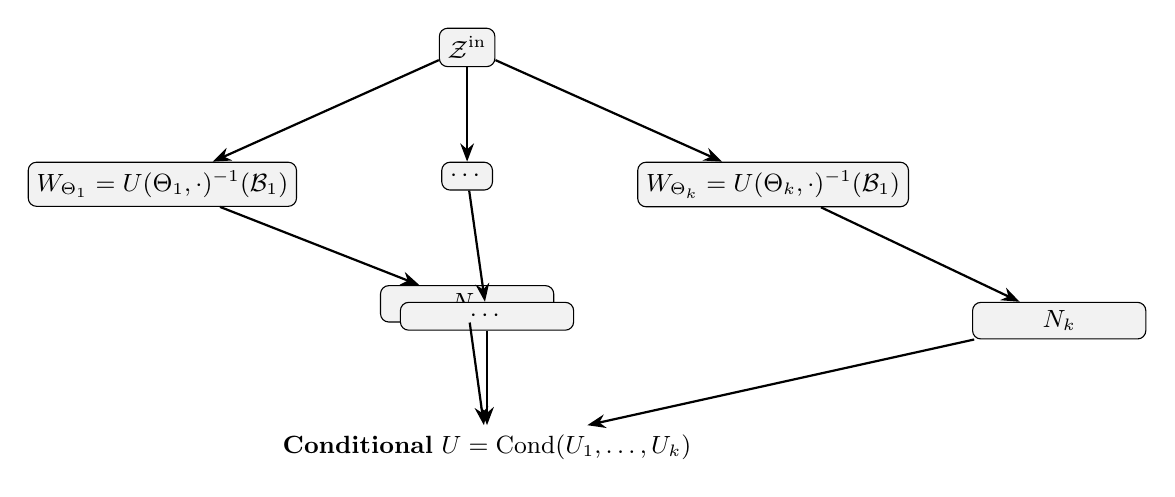
\begin{tikzpicture}[
  >=Stealth, node distance=1.8cm, font=\small,
  set/.style={draw, rounded corners=3pt, fill=gray!10, inner sep=3pt},
  arrow/.style={->, thick}
]
\node[set] (Zin) {$\mathcal Z^{\rm in}$};
\node[set, below left=1.2cm and 1.8cm of Zin] (W1) {$W_{\Theta_1}=U(\Theta_1,\cdot)^{-1}(\mathcal B_1)$};
\node[set, below=1.2cm of Zin] (W2) {$\cdots$};
\node[set, below right=1.2cm and 1.8cm of Zin] (Wk) {$W_{\Theta_k}=U(\Theta_k,\cdot)^{-1}(\mathcal B_1)$};

\draw[arrow] (Zin) -- (W1);
\draw[arrow] (Zin) -- (W2);
\draw[arrow] (Zin) -- (Wk);

\node[set, below=1.2cm of W2, minimum width=2.2cm] (N1) {$N_1$};
\node[set, below left=1.2cm and 0.8cm of Wk, minimum width=2.2cm] (N2) {$\cdots$};
\node[set, below right=1.2cm and 0.8cm of Wk, minimum width=2.2cm] (Nk) {$N_k$};

\draw[arrow] (W1) -- (N1);
\draw[arrow] (W2) -- (N2);
\draw[arrow] (Wk) -- (Nk);

\node[below=1.2cm of N2] (cond) {\textbf{Conditional} $U=\mathrm{Cond}(U_1,\dots,U_k)$};

\draw[arrow] (N1) -- (cond);
\draw[arrow] (N2) -- (cond);
\draw[arrow] (Nk) -- (cond);

\end{tikzpicture}
\caption{Open‑preimage gives an open cover $\{W_{\Theta_i}\}$; compactness $\Rightarrow$ finite subcover; refinement $\Rightarrow$ disjoint partition $\{N_i\}$; restriction $\Rightarrow$ sub‑maps $U_i$, assembled via Conditional.}
\end{figure}

\subsection{Edge Cases and Necessity Remarks}
\label{subsec:edge-cases}

\begin{remark}[If Nonemptiness Fails]
If for some $\Theta$, $U(\Theta,\cdot)^{-1}(\mathcal B_1)=\varnothing$, then no admissible input exists to ensure forward‑closure at tick 0.  Any certificate would be unsound or incomplete.  Thus nonemptiness is necessary.

\end{remark}

\begin{remark}[If Openness Fails]
If $U(\Theta,\cdot)^{-1}(\mathcal B_1)$ is nonempty but has empty interior (e.g., a fractal dust), then robustness collapses: infinitesimal noise can kick the system out of the admissible region.  Moreover, one generally needs infinitely many “hairline” cells to cover $\mathcal Z^{\rm in}$.  Finite tick‑0 decomposition fails, showing openness is necessary for our finite guarded construction.

\end{remark}

\begin{remark}[Beyond Tick 0]
The same equivalence holds shell‑by‑shell (Section~\ref{sec:inductive-shell-loop}): open‑preimage at every $n$ allows inductive refinement and a Loop‑Until construction.  Conversely, any such finite inductive decomposition implies open‑preimage at each level.

\end{remark}

\section{Inductive (Shell‑by‑Shell) Decomposition \& Loop‑Until}
\label{sec:inductive-shell-loop}

In this section we push the finite tick‑0 decomposition (Theorem~\ref{thm:op-iff-finite}) through \emph{all} certification shells.  We show how to refine guarded branches level by level and then wrap the whole tree into a single primitive we call \emph{Loop‑Until}.  This yields a programmatic update map that halts exactly when the state enters the invariant basin $\mathcal B$ (or a target shell $\mathcal B_N$).  The construction is inductive, quantitatively controlled by the Certification Standard $\mathcal S$, and qualitatively guaranteed by the Input‑Traceability axiom (Axiom~\ref{ax:open-preimage}).

%----------------------------------------------------------
\subsection{Setup and Notation}
\label{subsec:inductive-setup}

Recall:
\begin{itemize}
  \item $\mathcal S=\{\varepsilon_n\}_{n\ge1}$ is the minimal Certification Standard and
        $\mathcal B_n=\{\Theta:\operatorname{dist}(\Theta,\mathcal B)\le\varepsilon_n\}$ the $n$‑th shell.
  \item Axiom~\ref{ax:open-preimage} holds for \emph{every} shell: for all $n$ and $\Theta$,
        $U(\Theta,\cdot)^{-1}(\mathcal B_n)$ is open and nonempty.
  \item By Theorem~\ref{thm:op-iff-finite}, each shell admits a finite tick‑0 guarded decomposition.
\end{itemize}

We denote by $I_n$ the index set of all leaves (cells) at depth $n$ of the decomposition tree and by
\[
  \{\,N^{(n)}_{\mathbf i}\mid \mathbf i=(i_1,\dots,i_n)\in I_n\,\}
\]
the corresponding open cells ($\bigsqcup_{\mathbf i\in I_n} N^{(n)}_{\mathbf i}=\mathcal Z^{\rm in}$).  The restricted maps are
\[
  U^{(n)}_{\mathbf i}
  := U\ \big|_{\mathcal M\times N^{(n)}_{\mathbf i}}.
\]

%----------------------------------------------------------
\subsection{Inductive Refinement Lemma}
\label{subsec:inductive-lemma}

\begin{lemma}[Shell‑by‑Shell Refinement]
\label{lem:shell-refine}
Assume Axiom~\ref{ax:open-preimage} for $\mathcal B_{n+1}$.  
Suppose at level $n$ we already have a finite guarded decomposition
\[
  \{N^{(n)}_{\mathbf i},\ U^{(n)}_{\mathbf i}\}_{\mathbf i\in I_n}
\]
such that every leaf admits a nontrivial input guard‑band into $\mathcal B_n$.  Then there exists a finite refinement
\[
  \{N^{(n+1)}_{\mathbf i,j},\ U^{(n+1)}_{\mathbf i,j}\}_{(\mathbf i,j)\in I_{n+1}}
\]
of each leaf $\mathbf i\in I_n$ into children indexed by $j$, with:
\begin{enumerate}
  \item $N^{(n+1)}_{\mathbf i,j}\subseteq N^{(n)}_{\mathbf i}$ and $\bigcup_j N^{(n+1)}_{\mathbf i,j}=N^{(n)}_{\mathbf i}$ (disjoint open partition);
  \item $U^{(n+1)}_{\mathbf i,j}=U^{(n)}_{\mathbf i}\big|_{\mathcal M\times N^{(n+1)}_{\mathbf i,j}}$;
  \item Each child admits a nontrivial input guard‑band into $\mathcal B_{n+1}$.
\end{enumerate}
\end{lemma}

\begin{proof}
Fix a leaf $\mathbf i\in I_n$.  
By hypothesis, $(U^{(n)}_{\mathbf i},N^{(n)}_{\mathbf i})$ forwards $\mathcal B_n$ robustly.  
To refine to $\mathcal B_{n+1}\subseteq\mathcal B_n$, consider for any $\Theta$ the preimage
\[
  W_{\mathbf i,\Theta}^{(n+1)}
  := \bigl(U^{(n)}_{\mathbf i}(\Theta,\cdot)\bigr)^{-1}(\mathcal B_{n+1})
  \subseteq N^{(n)}_{\mathbf i}.
\]
Axiom~\ref{ax:open-preimage} (applied to $U^{(n)}_{\mathbf i}$, which equals $U$ on $N^{(n)}_{\mathbf i}$) says $W_{\mathbf i,\Theta}^{(n+1)}$ is open and nonempty for all $\Theta$. The family $\{W_{\mathbf i,\Theta}^{(n+1)}\}_{\Theta\in\mathcal M}$ covers $N^{(n)}_{\mathbf i}$. Compactness of $N^{(n)}_{\mathbf i}$ gives a finite subcover, which we refine to a disjoint open partition $\{N^{(n+1)}_{\mathbf i,j}\}_j$. Restrict $U^{(n)}_{\mathbf i}$ to each child to get $U^{(n+1)}_{\mathbf i,j}$.

By construction, for each $\Theta$, 
\[
  U^{(n+1)}_{\mathbf i,j}(\Theta,z)\in\mathcal B_{n+1}
  \quad\text{for all }z\in N^{(n+1)}_{\mathbf i,j}
\]
(or at least on a nonempty interior subset, depending on how we trimmed the cells), so the input guard‑band 
\(
  G^{\rm in,(n+1)}_{\mathbf i,j}(\Theta)
\)
has nonempty interior. This satisfies (3).  
Items (1)–(2) are by construction.  
\end{proof}

%----------------------------------------------------------
\subsection{Inductive Decomposition Theorem}
\label{subsec:inductive-decomp-theorem}

\begin{theorem}[Inductive Guarded Decomposition]
\label{thm:inductive-decomposition}
Assume \textbf{UI-Traceability} for every shell $\mathcal B_n$ (equivalently: Axiom~\ref{ax:open-preimage} holds and $\bigcup_{\Theta}U(\Theta,\cdot)^{-1}(\mathcal B_n)=\mathcal Z^{\mathrm{in}}$). 

Then for every $n$ there exists a finite family $\{N^{(n)}_{\mathbf i}, U^{(n)}_{\mathbf i}\}_{\mathbf i\in I_n}$ such that:
\begin{enumerate}
  \item $\{N^{(n)}_{\mathbf i}\}_{\mathbf i}$ is a disjoint open partition of $\mathcal Z^{\rm in}$;
  \item On each cell, $U^{(n)}_{\mathbf i}=U|_{\mathcal M\times N^{(n)}_{\mathbf i}}$;
  \item Each $U^{(n)}_{\mathbf i}$ admits a nontrivial input guard‑band into $\mathcal B_n$;
  \item The depth‑$n$ map is obtained by nesting conditionals:
  \[
    U^{(n)}=\mathrm{Conditional}\bigl(\{U^{(n)}_{\mathbf i}\}_{\mathbf i\in I_n}\bigr)
    \quad\text{and equals }U\text{ on }\mathcal M\times\mathcal Z^{\rm in}.
  \]
\end{enumerate}
\end{theorem}

\begin{proof}
By Theorem~\ref{thm:op-iff-finite} we have the base case $n=1$.  

For the base case $n=1$, apply Lemma~\ref{lem:no-crossing-from-minimal} to the finite tick-$1$ partition obtained from Theorem~\ref{thm:op-iff-finite} to extract, for each branch $N_i$, a certified input core $C_{1,i}$ with margin $\varepsilon_{1,i}>0$. This guarantees the guarded structure required for the Conditional primitive, ensuring that no certified trajectory starting in $C_{1,i}$ can cross $\partial N_i$ in one step.


Assume the statement for depth $n$; apply Lemma~\ref{lem:shell-refine} to every leaf to obtain the depth $n+1$ family.  The nested Conditional just stacks the new branch level under each leaf.  Induction completes the proof.
\end{proof}

\noindent\textbf{Comment.}
The theorem constructs a finite \emph{tree} of guarded sub‑maps for every shell.  Depth $n$ corresponds to staying safely within $\mathcal B_n$ in one step.  To actually \emph{stay} in the shell over time or to \emph{enter} $\mathcal B$, we need to iterate this tree until the state is inside $\mathcal B$.  That is the job of \emph{Loop‑Until}.


%----------------------------------------------------------
\subsection{Algorithmic View and Pseudocode}
\label{subsec:pseudocode}

For intuition, here is an abstract pseudocode embedding the inductive tree:

\begin{quote}
\textbf{Loop‑Until$(\Theta_0)$}\\
$n \leftarrow 1$\\
\textbf{while} $\Theta \notin \mathcal B$ \textbf{do}\\
\quad choose cell $N^{(n)}_{\mathbf i}$ s.t.\ $z\in N^{(n)}_{\mathbf i}$\\
\quad $\Theta \leftarrow U^{(n)}_{\mathbf i}(\Theta,z)$\\
\quad $n \leftarrow n+1$ \hfill // advance shell index (optional policy)\\
\textbf{end while}\\
\textbf{return} $(\Theta, n)$
\end{quote}

All the “choices” are guarded by the preimage openness, so every admissible $z$ keeps you inside the current shell.  Determinism is retained because $U$ is fixed and $z$ is the actual input; the branch selection is implicit in $(\Theta,z)$ landing in a unique cell $N^{(n)}_{\mathbf i}$.

%----------------------------------------------------------
\subsection{Diagram: Nested Conditionals + Loop}
\label{subsec:diagram-loop}

\begin{figure}[h!]
\centering
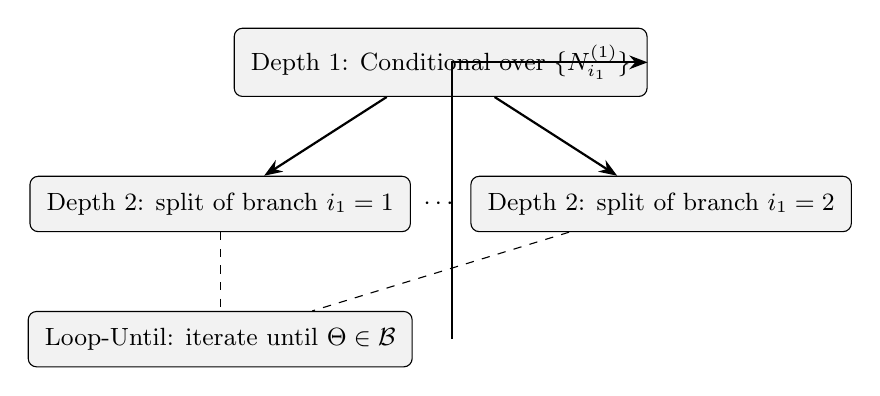
\begin{tikzpicture}[
  >=Stealth, node distance=1.2cm, font=\small,
  block/.style={draw, rectangle, rounded corners=3pt, fill=gray!10, inner sep=6pt},
  arrow/.style={->, thick}
]
\node[block] (lvl1) {Depth 1: Conditional over $\{N^{(1)}_{i_1}\}$};
\node[block, below=1.0cm of lvl1, xshift=-2.8cm] (lvl2l) {Depth 2: split of branch $i_1=1$};
\node[block, below=1.0cm of lvl1, xshift= 2.8cm] (lvl2r) {Depth 2: split of branch $i_1=2$};
\node (dots) at ($(lvl2l)!0.5!(lvl2r)$) {$\cdots$};
\node[block, below=1.0cm of lvl2l] (loop) {Loop‑Until: iterate until $\Theta\in\mathcal B$};

\draw[arrow] (lvl1) -- (lvl2l);
\draw[arrow] (lvl1) -- (lvl2r);
\draw[dashed] (lvl2l) -- (loop);
\draw[dashed] (lvl2r) -- (loop);
\draw[arrow] (loop.east) ++(0.5,0) |- (lvl1.east);

\end{tikzpicture}
\caption{A schematic: first a finite Conditional at depth 1, then each branch is refined at depth 2, etc.  The \emph{Loop‑Until} primitive iterates the nested tree until the basin is reached.  Dashed arrows indicate repeated traversal across depths.}
\end{figure}

%----------------------------------------------------------
\subsection{Edge Cases and Precision Targets}
\label{subsec:edge-precision}

\begin{remark}[Stopping at a Precision Shell]
Sometimes one wants to stop not at $\mathcal B$ itself, but when $L(\Theta)\le \delta$, i.e.\ $\Theta\in\mathcal B_{N(\delta)}$.  The same construction works with target shell $N(\delta)$ chosen so that $\varepsilon_{N(\delta)}\le \delta$.  Loop‑Until halts when $f(\Theta)\le N(\delta)$.
\end{remark}

\begin{remark}[Adaptive Shell Policies]
Instead of strictly incrementing $n$, one can keep $n$ fixed until the state is in $\mathcal B_n$, then jump to the next $n$.  Both policies produce a finite run.  The chosen policy affects $T_{\max}$ by at most a constant factor controlled by the shell gaps.
\end{remark}

\begin{remark}[If Axiom~\ref{ax:open-preimage} Fails at Some Level]
If open‑preimage holds up to shell $N$ but fails at $N\!+\!1$, the inductive refinement stops there.  You can still certify up to $\mathcal B_N$, but cannot guarantee further tightening.  This delineates the boundary of deterministic certifiability for that system.
\end{remark}

\section{Conclusion}
In this Chapter, we completed the following:

\begin{enumerate}
    \item \textbf{Deriving the Primitive Toolkit.}  
        We showed that \textsc{Sequential}, \textsc{Conditional}, and \textsc{Loop} suffice to build any valid composite test.  Their use is \emph{not} arbitrary: open-preimage (input traceability) and minimal standards regulate every branch and loop.
  \item \textbf{Open-Preimage $\Longleftrightarrow$ Finite Tick-0 Decomposition.}  
        The \textbf{\textit{traceability axiom}} is exactly the requirement that certification constraints lift to open, non-degenerate input sets.  With compactness, this gives a \emph{finite} guarded partition at tick~0.
  \item \textbf{Inductive Shell Decomposition \& Loop-Until.}  
        Shell-by-shell refinement—driven solely by $\mathcal S$—plus a terminating loop yields a total guarded program.  No extra geometry beyond continuity and compactness is needed.
\end{enumerate}

The ontological results of the Chapter are deep. After the Certification Standard appeared in the theory naturally (Book II, Chapter 6), we see the natural appearance of the next cornerstone concept of metrology - the \textbf{\textit{traceability}}. Again, nothing was introduced ad hoc here: it is a necessary consequence of the equivalence of the Simple Test to its decomposition.

\subsubsection{What's next?}
What we know now is that every Simple Test can be equivalently presented as a decomposition into the structure of tests guided by traceability requirement.

Our immediate next goal is to establish properties of the obtained decomposition. First question - if we achieved our goal of the creation of Turing Machine? And the second - how we can be sure it will eventually halt, producing our measurement result?

\end{document}